\documentclass[twocolumn, 10pt,a4j]{jsarticle}
% \documentclass[10pt,a4j]{jsarticle}
\usepackage{amsmath}
\usepackage[dvipdfmx]{graphicx}
\usepackage{url}
\usepackage{listings,jlisting} %日本語のコメントアウトをする場合jlistingが必
\usepackage{here}
\lstset{
  basicstyle={\ttfamily},
  identifierstyle={\small},
  commentstyle={\smallitshape},
  keywordstyle={\small\bfseries},
  ndkeywordstyle={\small},
  stringstyle={\small\ttfamily},
  frame={tb},
  breaklines=true,
  columns=[l]{fullflexible},
  numbers=left,
  xrightmargin=0zw,
  xleftmargin=3zw,
  numberstyle={\scriptsize},
  stepnumber=1,
  numbersep=1zw,
  lineskip=-0.5ex
}

% プリアンブル
\title{\vspace{-2.5cm}画像処理の基礎}
\author{T班 1610581 堀田 大地}
\date{2018/12/27}
\begin{document}
\maketitle{}
\section{目的}
% 目的
画像処理の基礎実装を通して,画像処理について学んだ.

\section{課題1 画素値と画像の関係}
  画素値によって色がどのように変化したかを確認した.
  \subsection{方法}
  \#1の部分に[1,255]の値を代入して確認した.
\begin{lstlisting}[caption=kadai1.py, label=p4_txt]
gazo = zeros((10,10))
for x in range(10):
    for y in range(10):
        gazo[y][x] = 255 #1
\end{lstlisting}

  \subsection{結果と考察}
    % 結果
    値が小さくなるにつれて黒に近づいた. これは,RGB要素を加法混色によって混ぜ合わせて色を生成しているからである.
    \begin{figure}[H]
    \begin{center}
        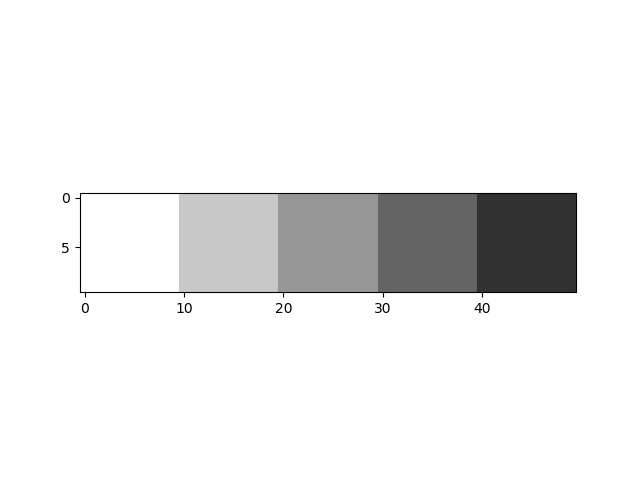
\includegraphics[width=7cm]{../img/kadai_1_value.png}
        \caption{値と色の関係. 右にいくにつれて値が小さくなっていっている.}
    \end{center}
    \end{figure}

\section{課題2 画素位置と画像の関係}
    配列のインデックスの数字と画像との対応を確認した.
    
    \subsection{方法}
\begin{lstlisting}[caption=kadai2.py, label=p4_txt]
gazo = zeros((10,10))
gazo[3][7] = 255
gazo_1[7][3] = 255
gazo_2[2][5] = 255
gazo_3[5][2] = 255
\end{lstlisting}
        
    \subsection{結果と考察}
    図2に上記のソースコードの結果を示す. 1次元目が$y$軸,2次元目が$x$軸に対応していた. 原点は左上で図形右側に$x軸$,下側に$y$軸の正の方向があった.
    % 図2
    \begin{figure}[H]
    \begin{center}
        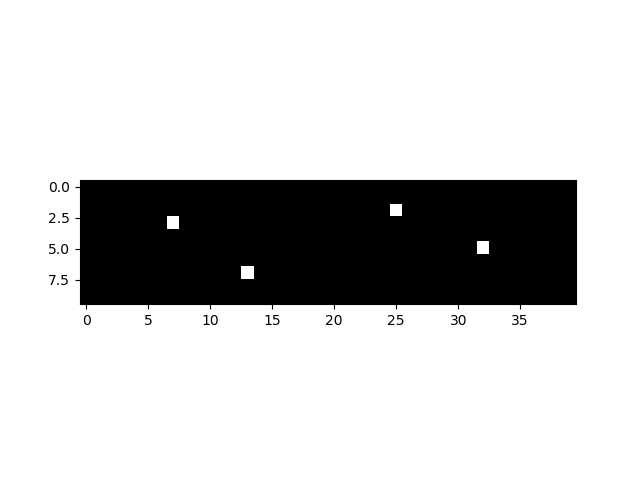
\includegraphics[width=7cm]{../img/kadai_2.png}
        \caption{画像の任意座標に255(白色)を代入した結果. 左からgazo, gazo1, gazo2, gazo3に対応する.}
    \end{center}
    \end{figure}

\section{課題3 図形の描画}
輪郭が黒く,その内側の領域が白い正方形を生成した.

    \subsection{方法}


\begin{lstlisting}[caption=kadai3.py, label=p4_txt]
gazo = zeros((10,10))
for x in range(10):
    for y in range(10):
        if 0 < x < 9 and 0 < y < 9:
            gazo[y][x] = 255
\end{lstlisting}
        
    \subsection{結果と考察}
    結果を図3に示した. $x,y$軸が[1,8]である場合に255を代入した.


    % 図3
    \begin{figure}[H]
    \begin{center}
        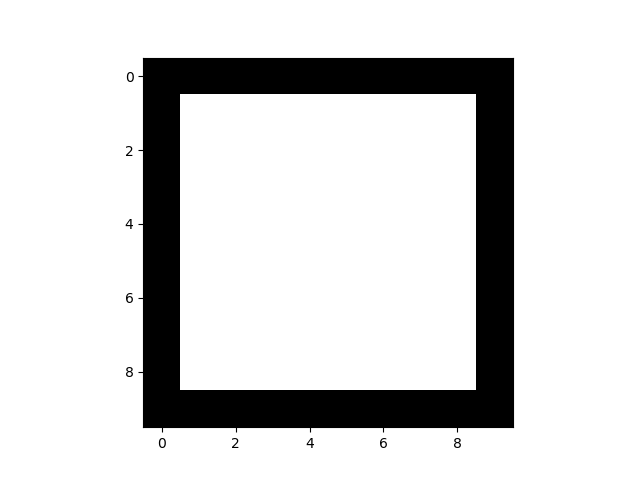
\includegraphics[width=7cm]{../img/kadai_3.png}
        \caption{輪郭が黒くその内側の領域が白い正方形.}
    \end{center}
    \end{figure}

\section{課題4 フィルタ}
移動平均フィルタ,ラプラシアンフィルタを実装した.

    \subsection{方法}
    移動平均,ラプラシアンフィルタの実装のコードを載せた. 移動平均フィルタは自分の周囲9ピクセルの画素値の平均値を求めている. また,ラプラシアンフィルタは二次微分を利用して画像から輪郭を抽出している.

\begin{lstlisting}[caption=kadai4IdouHeikin.py, label=p4_txt]
gazo_idou = zeros((12,12))
for x in range(1,11):
    for y in range(1,11):
        filter = [
            [0.5, 0.5, 0.5],
            [0.5, 0.5, 0.5],
            [0.5, 0.5, 0.5]
            ]
        gasochi = 0
        for xx in range(3):
            for yy in range(3):
                gasochi += gazo[y+yy-1][x+xx-1] * filter[yy][xx]
        gasochi = int(gasochi) 
        if gasochi < 0:
            gasochi = 0
        elif gasochi > 255:
            gasochi = 255
        gazo_idou[y][x] = gasochi
\end{lstlisting}

\begin{lstlisting}[caption=kadai4Laplasian.py, label=p4_txt]
gazo_lap = zeros((12,12))
for x in range(1,11):
    for y in range(1,11):
        filter = [
            [0.0, 1.0, 0.0],
            [1.0, -4.0, 1.0],
            [0.0, 1.0, 0.0]
            ]
        gasochi = 0
        for xx in range(3):
            for yy in range(3):
                gasochi += gazo[y+yy-1][x+xx-1] * filter[yy][xx]
        gasochi = int(gasochi) 
        if gasochi < 0:
            gasochi = 0
        elif gasochi > 255:
            gasochi = 255
        gazo_lap[y][x] = gasochi
\end{lstlisting}


    \subsection{結果と考察}
        結果を図4に示す. 結果よりそれぞれの役割がわかった.
        \begin{enumerate}
            \item 移動平均フィルタ \\
                注目領域周囲9ピクセルの平均値をそこに代入している.
            \item ラプラシアンフィルタ \\
                カーネルの導出方法を示す. 水平方向および垂直方向の画素値の一次微分は(1),(2)で表せる. 加えて,二次微分は
                もう一度差分を取ることで(3),(4)で表せる.
                \begin{eqnarray}
                    I_{x}(x, y) &=& I(x+1, y) - I(x, y) \\
                    I_{y}(x, y) &=& I(x, y+1) - I(x, y) \\
                    I_{xx}(x, y) &=& I(x+1, y) - I(x, y) - I(x, y) - I(x -1, y) \nonumber \\ 
                    &=& I(x-1, y) - 2I(x, y) + I(x+1, y) \\
                    I_{yy}(x, y) &=& I(x, y-1) - I(x, y) - I(x, y) - I(x, y+1) \nonumber \\ 
                    &=& I(x, y-1) - 2I(x, y) + I(x, y+1)
                \end{eqnarray}

                よって,ラプラシアン$\nabla^2 I(x, y)$は(5)で表せれる.
                \begin{eqnarray}
                    \nabla^2 I(x, y) &=& I_{xx}(x, y) + I_{yy}(x, y) \nonumber \\
                    &=& I(x-1, y) + I(x, y-1) - 4I(x, y) \nonumber \\
                    &+& I(x+1, y) + I(x, y+1)
                \end{eqnarray}
        \end{enumerate}

        \begin{figure}[H]
            \begin{center}
                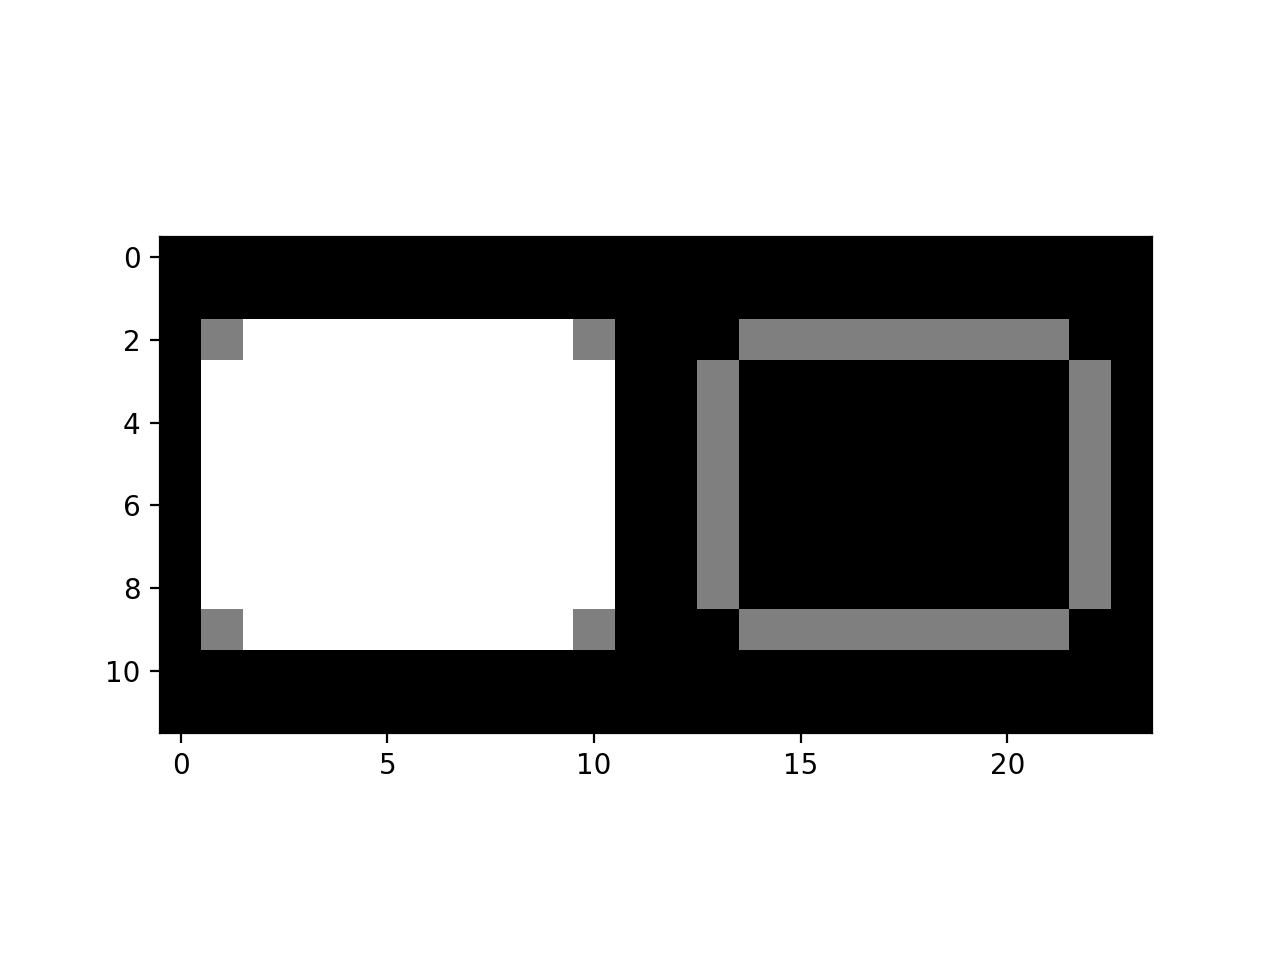
\includegraphics[width=7cm]{../img/Figure_2.png}
                \caption{左:移動平均フィルタの結果,右:ラプラシアンフィルタの結果.}
            \end{center}
            \end{figure}

\section{課題5 ヒストグラムと二値化}
    画像の特徴を表わす二値画像が生成されるように作成した.
        
    \subsection{方法}
    ピクセル毎に,ある閾値より下回る画素値であれば,0を代入,それ以外であれば255を代入した.

\begin{lstlisting}[caption=kadai5.py, label=p4_txt]
def shori(gazo, gazo2, SIKII):
    """
    Args:
        gazo : 入力画像の配列.
        gazo2 : 出力画像の配列.
        SIKII : 閾値.
    """
    for x in range(gazo.shape[1]):
        for y in range(gazo.shape[0]):
            value = gazo[y][x]
            if value < SIKII:
                gazo2[y][x] = 0
            else:
                gazo2[y][x] = 255
    return gazo2
\end{lstlisting}

    \subsection{結果と考察}
    閾値が大きいと望んでいないノイズも含まれた. 


    \begin{figure}[H]
        \begin{center}
            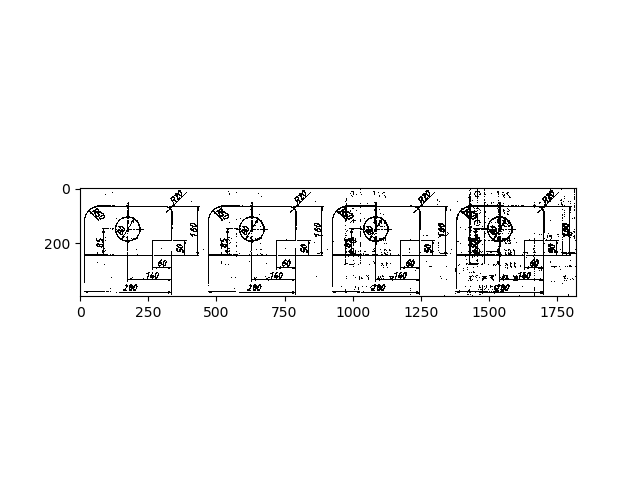
\includegraphics[width=7cm]{../img/kadai_5.png}
            \caption{左から閾値が220,225,230,235の結果.}
        \end{center}
        \end{figure}

\section{課題6 ヒストグラムと階調変換}
濃淡がよりはっきりとする画像を生成した.

    \subsection{手法}
    画像の正規化を行なった. また,平均輝度と輝度値の標準偏差は好みで決めた.

\begin{lstlisting}[caption=kadai5.py, label=p4_txt]
def tra(img, mean_kido, std):
    """
    Args:
        img : 入力画像.
        mean_kido : 平均輝度.
        std : 輝度値の標準偏差.
    """
    img = (img - np.mean(img))/np.std(img)*std + mean_kido
    return img
\end{lstlisting}


    \subsection{結果と考察}
    結果は図6,7のようになった. 正規化を行うことで濃淡がはっきりとした.
    \begin{figure}[H]
        \begin{center}
            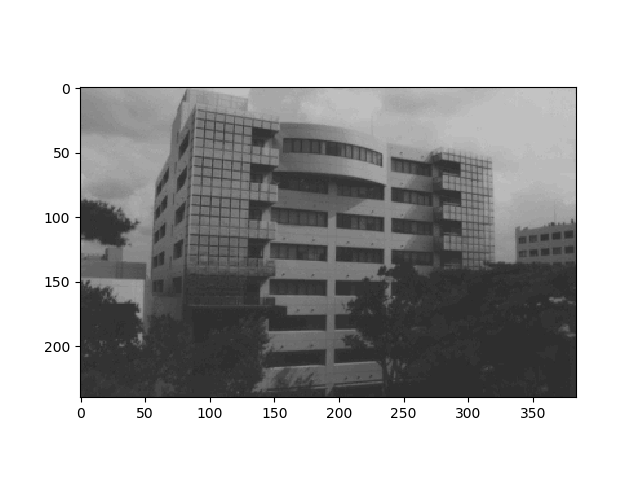
\includegraphics[width=7cm]{../img/result_fig.png}
            \caption{平均輝度100, 輝度値の標準偏差50の画像.}
        \end{center}
        \end{figure}

        \begin{figure}[H]
            \begin{center}
                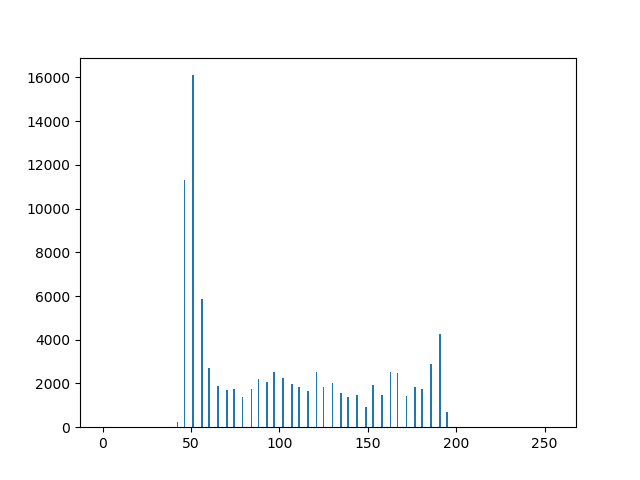
\includegraphics[width=7cm]{../img/result_hist.png}
                \caption{図6の画素値のヒストグラム.}
            \end{center}
            \end{figure}


\section{課題7 図形の面積の計算}
図8中の6つの図形の面積,つまり画素数,を計算した.
\begin{figure}[H]
    \begin{center}
        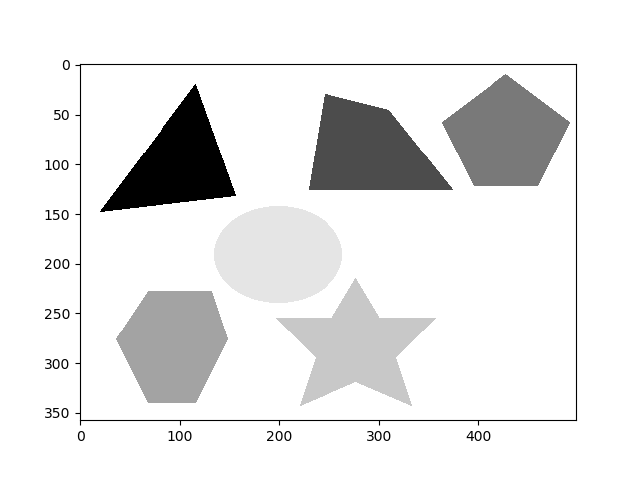
\includegraphics[width=7cm]{../img/kadai_7.png}
        \caption{面積を求める画像.}
    \end{center}
    \end{figure}

    \subsection{手法}
    画素値集合を取って,どの画素値があるか把握した上で,その画素値の数をカウントして求めた.
\begin{lstlisting}[caption=kadai7.py, label=p4_txt]
uniq = unique(gazo)
result = {
    uniq[0]:0,
    uniq[1]:0,
    uniq[2]:0,
    uniq[3]:0,
    uniq[4]:0,
    uniq[5]:0,
    uniq[6]:0
    }
for y in range(0,358):
    for x in range(0,499):
        value = gazo[y][x]
        if value == uniq[0]:
           result[uniq[0]] +=1
        elif value == uniq[1]:
           result[uniq[1]] +=1
        elif value == uniq[2]:
           result[uniq[2]] +=1
        elif value == uniq[3]:
           result[uniq[3]] +=1
        elif value == uniq[4]:
           result[uniq[4]] +=1
        elif value == uniq[5]:
           result[uniq[5]] +=1
        elif value == uniq[6]:
           result[uniq[6]] +=1
\end{lstlisting}


\subsection{結果と考察}
結果を表1に示した. 
\begin{table}[htb]
    \caption{図8の各図形の面積.}
    \begin{tabular}{ccc}
      図形 & 面積 & 画素値  \\ \hline
      三角形 & 8145 & 0 \\
      台形 & 9185 & 76 \\
      五角形 & 9265 & 200 \\
      六角形 & 9425 & 122 \\
      星 & 9545 & 164 \\
      丸 & 9841 & 229
    \end{tabular}
  \end{table}

\subsection{課題8 図形の輪郭線の長さの計算}
画像8中の各図形の輪郭線の長さを計算した.


  \subsection{手法}
ラプラシアンフィルタを用いて輪郭抽出を行う. しかしながら,ただ輪郭抽出を行うだけだと
各図形の輪郭線の画素値が均一でないため課題7のように数えあげることができない. なので,
なので次の手順で輪郭の長さを計算した.
\begin{enumerate}
    \item 入力画像$A$からラプラシアンフィルタを用いて輪郭線の画素値を0,その他の部分を255にした画像$B$を作成した. \\
    \item $C = |B - A|$を求めて,各図形の画素値が均一でないことを利用して,輪郭線画素値を不均一にした. \\
    \item $D = |C - A|$を求めて,輪郭内部の画素値を0にした. つまり,輪郭線以外の画素値は0である. \\
    \item 課題7と同様に,各輪郭線の長さを求めた.
\end{enumerate}

  \begin{figure}[H]
    \begin{center}
        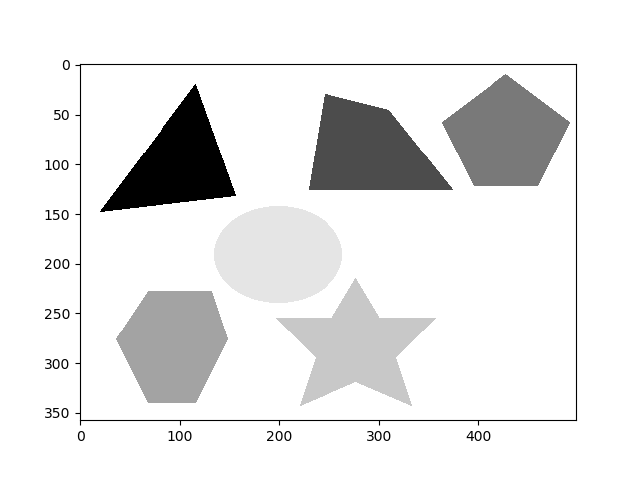
\includegraphics[width=7cm]{../img/kadai_7.png}
        \caption{輪郭だけを持つ図形.}
    \end{center}
    \end{figure}

  \subsection{結果と考察}
  結果を表2に示した. ラプラシアンフィルタは周りの画素を用いて計算するので,当然条件によって
  輪郭線の画素値は変わってくるので,前処理を施した.
    
  \begin{table}[htb]
    \caption{図8の各輪郭線の長さ.}
    \begin{tabular}{ccc}
      図形 & 長さ  \\ \hline
      三角形 & 276 \\
      台形 & 320 \\
      五角形 & 320 \\
      六角形 & 336 \\
      星 & 384 \\
      丸 & 480
    \end{tabular}
  \end{table}

\section{結論}
画像処理の基礎実装を通して,画像処理について学ぶことができた. さらに,課題8では画像の
前処理を考えることで,フィルタ演算だけではできない計算を行うことを学んだ.

\section{感想}
  ディスプレイを濡れたティッシュで掃除すると3色に輝いてたのはとても面白かった.
\end{document}